\documentclass[12pt,a4paper]{article}

\usepackage[T1]{fontenc}
\usepackage[brazilian]{babel}
\usepackage{lmodern}
\usepackage[margin=2.5cm]{geometry}
\usepackage{amsmath}
\usepackage{amssymb}
\usepackage{graphicx}
\usepackage{booktabs}
\usepackage{microtype}
\usepackage{natbib}
\usepackage{float}
\usepackage[hidelinks]{hyperref}

\title{Análise Mensal de Temperatura do Ar}
\author{Thiago Saddock}
\date{\today}

\begin{document}

\maketitle

\section{Origem dos Dados}
\label{sec:dados}

\hspace{\parindent}Os dados utilizados neste relatório provêm do conjunto \texttt{airquality}, nativo da linguagem de programação R \citep{rcore}. O arquivo analisado contém um total de 153 observações. A análise foca na variável \texttt{Temp} que indica a temperatura do ar

Para visualizar a distribuição dessa variável ao longo do tempo, foi gerado a Figura~\ref{fig:distribuicao} utilizando as ferramentas gráficas do R, com o auxílio do pacote \texttt{ggplot2} \citet{ggplot2}.

\begin{figure}[htbp]
  \centering
  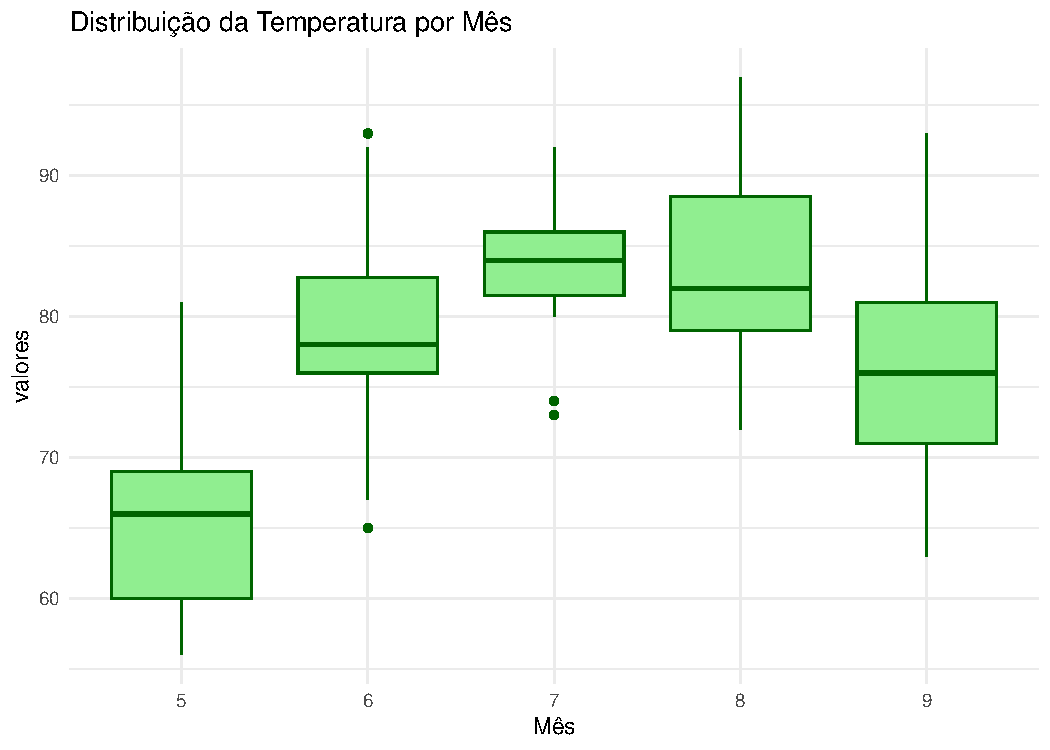
\includegraphics[width=0.7\textwidth]{figura.pdf}
  \caption{Distribuição da Temperatura ao longo dos cinco meses observados.}
  \label{fig:distribuicao}
\end{figure}

\section{Resultados e Metodologia}
\label{sec:resultados}

\hspace{\parindent}Conforme indicado pela Tabela~\ref{tab:resumo}, foi calculado a média mensal da variável. 

\begin{table}[H]
  \centering
  \caption{Média mensal e dias de medição.}
  \label{tab:resumo}
  \begin{tabular}{lrr}
    \toprule
    Mês & Média & Dias Medidos \\
    \midrule
    5 & 65,55 & 31 \\
    6 & 79,10 & 30 \\
    7 & 83,90 & 31 \\
    8 & 83,97 & 31 \\
    9 & 76,90 & 30 \\
    \bottomrule
  \end{tabular}
\end{table}

A média por mês apresentada na Tabela~\ref{tab:resumo} foi obtida por meio da Equação~\eqref{eq:media}:

\begin{equation}
  \label{eq:media}
  \bar{x} = \frac{1}{n} \sum_{i=1}^{n} x_i
\end{equation}

Nesta equação, o denominador $n$ não representa o total absoluto de dias do mês, mas sim estritamente o número de dias em que houve medição válida, ignorando os valores ausentes (NA) detectados no arquivo.

\section*{Declaração de uso de IA}

\hspace{\parindent}Utilizei modelos de inteligência artificial generativa (Gemini) para auxiliar na sintaxe de rotinas bash, na refatoração do código R (para uso correto de ferramentas de linting) e na estruturação do documento LaTeX. Todos os retornos lógicos e de formatação foram validados rodando o código em terminal e comparando a saída com as exigências da atividade.

\bibliographystyle{plainnat}
\bibliography{referencias}

\end{document}